In this section, we provide a short description of Spark Streaming's architecture as well as relevant terminologies needed to understand our work.

\begin{figure}[t!]
  \begin{center}
    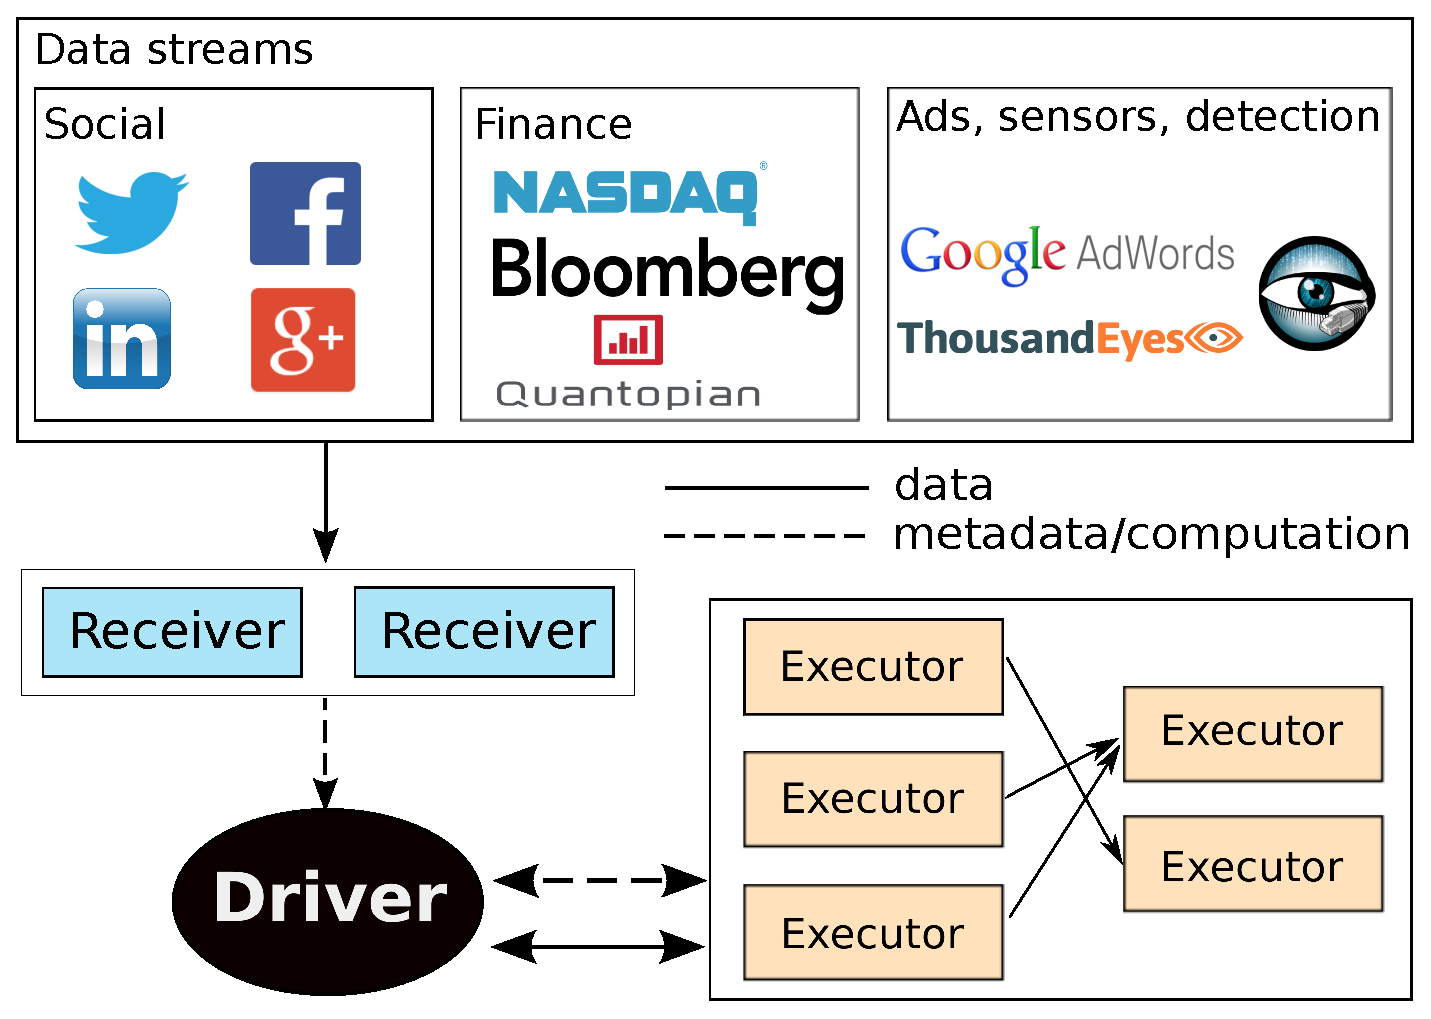
\includegraphics[scale=0.35]{images_graphs/spark_architecture_v4.eps}
  \end{center}
  \caption{Diagram of a Spark Streaming work flow. A Receiver and an Executor may execute in the same node.}
  \label{fig:SparkStreaming_architecture}
\end{figure}

Spark~\cite{Spark} is a general-purpose engine for large-scale cluster computing. It operates on Resilient Distributed Datasets (RDDs), an abstraction that represents read-only collections of objects partitioned across a set of machines. RDDs can be created from raw data or other RDDs, and keep track of the coarse-grained operations (e.g., \texttt{map}, \texttt{reduce}) performed on its underlying data as lineage information, so that partitions can be recomputed if they are lost due to failures. 
Another feature of RDDs is that they can be persisted in memory, allowing efficient iterative computations.

Spark Streaming, the focus of our work, is a stream processor built on top of Spark.
It implements an abstraction called discretized streams (D-Streams), which takes advantage of RDDs and their lineage properties to divide potentially infinite streams of data into finite chunks and provide an interface to perform computation over it.
The abstraction allows a micro-batch approach to streaming data, yielding high throughput, scalability and fault-tolerance.


The execution of a Spark Streaming job works as depicted in Figure~\ref{fig:SparkStreaming_architecture}. 
First, data is generated at a source (e.g., tweets from Twitter). As the data is pushed into Spark Streaming, it is received by a Receiver, which in turn stashes it in memory. After every set amount of time called the block interval, the Receiver takes the data stashed in memory and generates a block with it.

Once a block is generated, the Receiver informs a Spark Streaming's central component called Driver about this block. The Driver is responsible for holding metadata about reported blocks from all Receivers.
After a separate, larger fixed amount of time called the batch interval or batch window, the Driver takes all blocks that have been communicated by the Receivers and that have yet to be processed and generates a batch job with them. Generated jobs are passed to the Scheduler (not shown in diagram) to be scheduled and run on machines available in the cluster.

Every batch job is divided into one or more stages. Each stage can be a map stage or reduce stage. Stages have to be processed in sequence, so the more stages required for a job, i.e. the more reduce operations used by the application, the longer a job will take to execute.

Each stage operates on a RDD. The RDDs are partitioned by the blocks generated during the batch interval, and can be processed in parallel. The computation on a partition is called a task. Tasks are sent from the Scheduler to run in stateless environments called Executors. Executors are usually deployed in the same nodes as Receivers; in fact, Receivers are implemented as long-running tasks.

\begin{figure}[t!]
  \begin{center}
    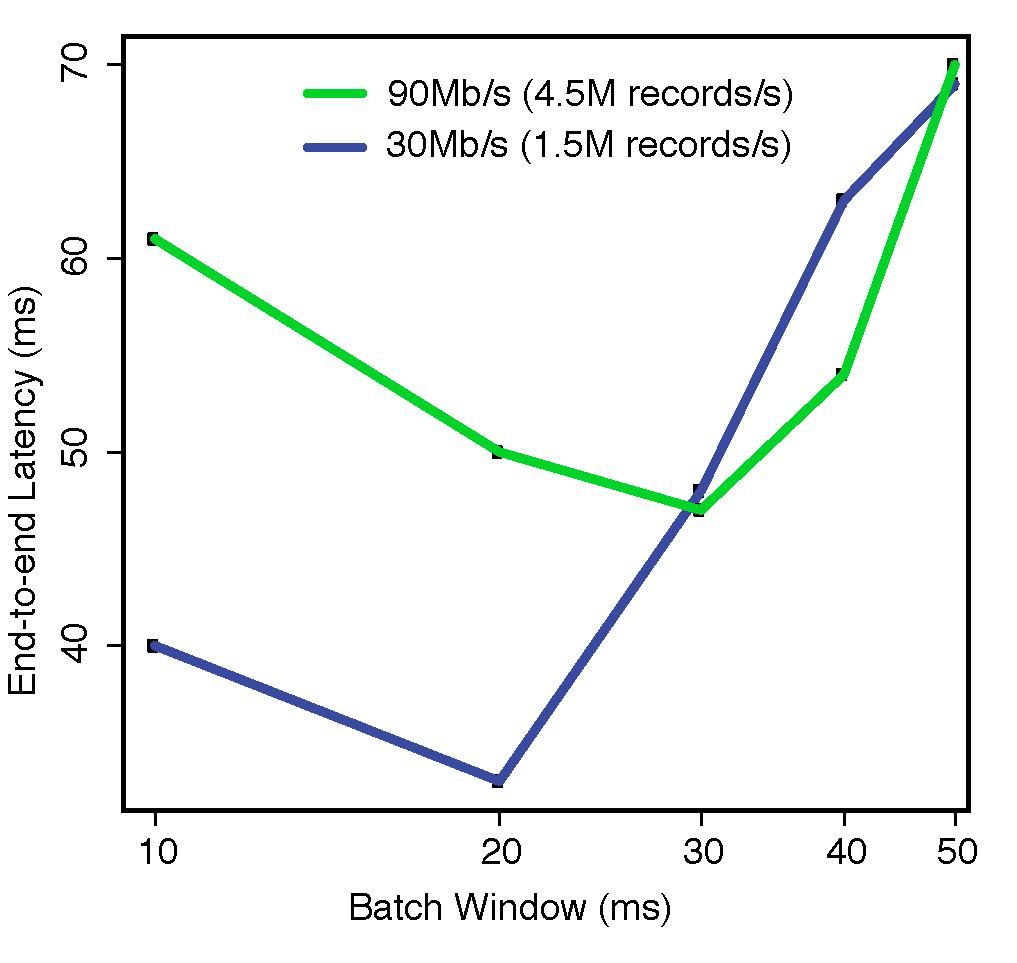
\includegraphics[scale=0.50]{images_graphs/batchsize_vs_latency/batchsize_vs_latency_illustrator.pdf}
  \end{center}
  \caption{Average end-to-end latency for different batch window sizes and different throughputs. For batch windows smaller than 10ms the average end-to-end latency tens to infinity.}
  \label{fig:Batchsize_vs_latency}
\end{figure}

At the heart of the micro-batch approach taken by Spark is the trade-off between the amount of records Spark can process per unit of time and the time the system takes to return results to the user.
On one hand, waiting for more records to generate bigger batches allows Spark Streaming to amortize its overheads. On the other hand, the more time the system waits for data, the less responsive the system becomes.
%Moreover, Spark can provide window semantics over data. For instance, a user can use Spark Streaming to compute the average temperature during the last 30 minutes over a stream of temperature sensor data.

%Internally, Spark Streaming makes extensive use of Actors -- a design pattern that decouples the invocation of methods from its execution. 
%In this approach, the invocation of methods between certain components is performed by inserting a message in a queue of the message receiver.
%The component that receives the message continuously polls the queue and services messages in parallel.
%This approach has been shown to provide high levels of concurrency and adaptability to changing loads~\cite{SEDA}.

Internally, Spark Streaming makes extensive use of the producer-consumer design pattern, where separate threads offload work to each other through queues. For example, as blocks are generated at the receiver, they are pushed to a queue by a producer thread. The corresponding consumer thread constantly polls the queue, and stores the dequeued block as well as sends metadata about the block to the Driver. As well, communications between different components of the system is done through the Actor model, where components (``actors") talk to each other by sending messages to each other's message queues.

